\documentclass[11pt,a4paper]{article}
\usepackage[utf8]{inputenc}
\usepackage{amsmath}
\usepackage{amsthm}
\usepackage{amsfonts}
\usepackage{amssymb}
%\usepackage{algorithmic}
%\usepackage{algorithm}
\usepackage{hyperref}
%\usepackage[ruled,linesnumbered,procnumbered]{algorithm2e}

\makeatletter
\let\original@algocf@latexcaption\algocf@latexcaption
\long\def\algocf@latexcaption#1[#2]{%
  \@ifundefined{NR@gettitle}{%
    \def\@currentlabelname{#2}%
  }{%
    \NR@gettitle{#2}%
  }%
  \original@algocf@latexcaption{#1}[{#2}]%
}
\makeatother

\usepackage{xcolor}		% for adding colors to the text

\usepackage[footnotesize, center]{caption}	
\usepackage{subcaption}
%\usepackage{subfigure}
\usepackage{booktabs}
\usepackage{multirow}
\usepackage{breakurl}	% fixes the problem of breaking long url into lines inside the bibliography (IMP: must be below the hyperref package)
\hypersetup{
    bookmarks=true,		% show bookmarks bar?
    colorlinks=true,		% false: boxed links; true: colored links
    linkcolor=blue,		% color of internal links
    citecolor=blue,		% color of links to bibliography
    filecolor=blue,		% color of file links
    urlcolor=blue,		% color of external links
    bookmarksopen=true,
    breaklinks=true,
}
%\usepackage{natbib}			% bibliography
%\setlength{\bibsep}{0pt}

\usepackage[title]{appendix}

\usepackage{longtable}

% Page Setup

% Margins
	% MS Word (Default):		[margin=0.98in]
	% MS Word (Narrow):		[margin=0.5in]
\usepackage[margin=2cm]{geometry}
\setlength{\parskip}{\medskipamount}

\usepackage{setspace}
%\onehalfspacing
\setstretch{1.15}

\usepackage{indentfirst}			% indent the first paragraph
\allowdisplaybreaks				% break if equations take too much vertical space

% Section Style
\makeatletter
\def\@seccntformat#1{\csname the#1\endcsname.\quad}		% put a fullstop after section numbers
\makeatother

% Optional packages
\usepackage{xfrac}	% nicer fractional symbols (e.g., \sfrac{1}{2})
\usepackage{fancyhdr}	% adding headers / footers

% MACROS

% mathematical
\newcommand{\mathbold}[1]{\boldsymbol{#1}}		% for adding bold greek letters
\newcommand{\binary}{\{ 0, 1 \} }

\newcommand{\parentheses}[1]{\left( #1 \right) }	% auto-size parentheses
\newcommand{\brackets}[1]{\left[ #1 \right] }		% auto-size brackets
\newcommand{\curly}[1]{\left\{ #1 \right\} }		% auto-size curly brackets

	% Nilay Noyan's commenting macros
	% commentbox (adds black comments in a frame box)
	% comment (adds red comments as a footnote)

\newcounter{commentcounter}
\setcounter{commentcounter}{1}

\setlength{\fboxsep}{5pt}
\setlength{\fboxrule}{0.1pt}

\newcommand{\commentbox}[1]{
% \hfill \newline \noindent
%	\framebox[\textwidth]{
%		\parbox{0.98\textwidth}{
%			\footnotesize{
%				\texttt{\textcolor{black}{(C.\arabic{commentcounter})~#1\hfill}}}}}
%	\addtocounter{commentcounter}{1} 
	}

\long\def\symbolfootnote[#1]#2{\begingroup\def\thefootnote{\fnsymbol{footnote}}\footnote[#1]{#2}\endgroup}

\newcommand{\comment}[2]{{\footnotesize\texttt{\textcolor{red}{(C.\arabic{commentcounter})}}\symbolfootnote[4]{\texttt{\textcolor{red}
        {(C.\arabic{commentcounter}) [#1]: ~#2}}}}\addtocounter{commentcounter}{1}}
%\newcommand{\comment}[2]{}

% theorems
% the subtheorem environment is used to generate theorem numbers 1a, 1b, etc.
% Source: http://tex.stackexchange.com/questions/43346/how-do-i-get-sub-numbering-for-theorems-theorem-1-a-theorem-1-b-theorem-2
\makeatletter
\newenvironment{subtheorem}[1]{%
  \def\subtheoremcounter{#1}%
  \refstepcounter{#1}%
  \protected@edef\theparentnumber{\csname the#1\endcsname}%
  \setcounter{parentnumber}{\value{#1}}%
  \setcounter{#1}{0}%
  \expandafter\def\csname the#1\endcsname{\theparentnumber\alph{#1}}%
  \ignorespaces
}{%
  \setcounter{\subtheoremcounter}{\value{parentnumber}}%
  \ignorespacesafterend
}
\makeatother
\newcounter{parentnumber}
% end of subtheorem environment

\newtheorem{theorem}{\bf Theorem}
\newtheorem{lemma}{\bf Lemma}
\newtheorem{proposition}{\bf Proposition}
\newtheorem{corollary}{\bf Corollary}
\newtheorem{definition}{\sc Definition}
\newtheorem{fact}{\bf Fact}
\newtheorem{claim}{\sc Claim}
\newtheorem{case}{\sc Case}
\newtheorem{observation}{\sc Observation}
\renewcommand{\qedsymbol}{\hfill \tiny$\blacksquare$}		% symbol for proof environment
\renewcommand{\proofname}{\textnormal{\textbf{Proof.}}}	% title in the proof environment

\newtheoremstyle{mytheoremstyle} % name
    {\topsep}                    % Space above
    {\topsep}                    % Space below
    {}                   % Body font
    {}                           % Indent amount
    {\scshape}                   % Theorem head font
    {.}                          % Punctuation after theorem head
    {.5em}                       % Space after theorem head
    {}  % Theorem head spec (can be left empty, meaning ‘normal’)
\theoremstyle{mytheoremstyle}
\newtheorem{example}{Example}

\newtheoremstyle{myassumptionstyle} % name
    {\smallskipamount}                    % Space above
    {0}                    % Space below
    {}                   % Body font
    {}                     	% Indent amount
    {\upshape}              % Theorem head font
    {.}                          	% Punctuation after theorem head
    {.5em}                      % Space after theorem head
    {}  				% Theorem head spec (can be left empty, meaning ‘normal’)
\theoremstyle{myassumptionstyle}
\newtheorem{assumption}{\bf A\ignorespaces}
\newtheorem{remark}{\bf Remark}

\DeclareMathOperator*{\argmin}{arg\,min} 
\DeclareMathOperator*{\argmax}{arg\,max} 


% narrative
\newcommand{\ie}{\textit{i.e.}}		% id est, that is to say
\newcommand{\ex}{\textit{ex.}}		% example
\newcommand{\eg}{\textit{e.g.}}	% exempli gratia, for the sake of example

\newcommand{\st}{\text{subject to:}\qquad}	% subject to
\newcommand{\mathbi}[1]{\boldsymbol{#1}}	% \boldsymbol{ any character } // makes both italic and bold

\newcommand{\cplex}{\texttt{CPLEX}}

\newcommand{\question}[1]{\vspace{\baselineskip}\noindent\pdfbookmark{Question #1}{Question #1}\textbf{\large{Question #1}} \normalsize\medskip\newline}
\newcommand{\qpart}[1]{\indent\textbf{#1)}}	% i.e., a), b), ...

\newcommand{\inlinecomment}[1]{{\color[rgb]{0.13,0.57,0.4} \textbf{#1}}}

% algorithmic
\newcommand{\np}{$\mathcal{NP}$}	% e.g., as in NP-hard

\usepackage{enumitem}	% for aligned descriptions
\usepackage{calc} 		% for aligned descriptions

\setenumerate{
itemsep=0pt,
partopsep=0pt,
parsep=0pt,
topsep=0pt,
labelindent=4pt,
font=\normalfont
}

\setdescription{
itemsep=0pt,
partopsep=0pt,
parsep=0pt,
topsep=0pt,
labelindent=4pt,
font=\normalfont
}

\setitemize{
itemsep=0pt,
partopsep=0pt,
parsep=0pt,
topsep=0pt,
labelindent=4pt,
font=\normalfont
}


\usepackage{natbib}			% bibliography
\setlength{\bibsep}{0pt}

\setlength{\textheight}{23cm} %{23cm}
\setlength{\topmargin}{-2cm}
\setlength{\textwidth}{17.5cm} \setlength{\oddsidemargin}{-0.5cm}
\setlength{\evensidemargin}{-0.5cm}

\setlength{\parindent}{0pt}

\newcommand{\gap}{\vspace{5pt}}
\newcommand{\epc}{\hspace{1pc}}

\newcommand{\onebld}{{\bf 1}}
\newcommand{\wt}{\widetilde}
\newcommand{\wh}{\widehat}

\usepackage{moreverb} % for verbatim ouput
% Count of words
\immediate\write18{texcount -inc -incbib 
-sum writeup.tex > /tmp/wordcount.tex}
\newcommand\wordcount{
\verbatiminput{/tmp/wordcount.tex}}

% Count of characters
\immediate\write18{texcount -char -freq
 writeup.tex > /tmp/charcount.tex}
\newcommand\charcount{
\verbatiminput{/tmp/charcount.tex}}

\newcommand{\E}{{\rm I\!E}}
\newcommand{\IP}{{\rm I\!P}}
\newcommand{\D}{{\rm I\!D}}
\newcommand{\pmat}[1]{\begin{pmatrix} #1 \end{pmatrix}}
\newcommand{\us}[1]{{\color{black}#1}}
\newcommand{\ssbs}[1]{{\color{blue}#1}}
\bibliographystyle{apalike}

\title{\bf Taming the Duck: Can Stochastic Programming Help?}

\begin{document}
\maketitle

\section{Intro that, potentially, should be dropped out}

\begin{itemize}
\item Furthermore, the biggest obstacle against the growth of renewable resources, namely their economies of scale, has been lowered due to new technological advances, leading the way for marked additions of renewable-capacity in recent years \citep{Guardian2017}. 
\item An engineer's perspective towards ever increasing share of renewables in power grids is not completely enthusiastic. The availability of renewable resources depends on nature, and harvesting solar and wind is not trivial, at least, in comparison to the extraction, storage, and burning of fossil-fuels. Accordingly, with increasing renewable integration, new challenges emerge in power systems that need to be addressed with caution, so that the efficiency and reliability of operations can be maintained. The goal of this chapter is to examine these challenges, and offer specific suggestions, primarily, in the context of power-system operations planning, and more specifically, planning under renewable uncertainty.
\end{itemize}

The organization of this chapter is as follows. In \S\ref{ch:td:sec:quandary}, we elaborate the adversities of renewable-energy resources which cause concern for some engineering communities. This section will also elucidate our choice of title for this chapter. Next, in \S\ref{ch:td:sec:models}, we provide a modeling framework for experimenting with daily power-system operations in typical grids. Then, we use this framework to conduct experiments in \S\ref{ch:td:sec:experiments} on a test grid. These experiments will reveal the challenges faced by the power industry, and assess the impact of algorithmic novelties to overcome the uncertain nature of renewable resources. Concluding remarks are given in \S\ref{ch:td:sec:notes}.

\section{The Quandary of Renewable Energy Integration} \label{ch:td:sec:quandary}

Lawmakers throughout the U.S. have mandated that a significant percentage of electricity supply should be derived from renewable resources --- each state has set its own goal, with California being the most aggressive, requiring 50\% by 2030 \citep{CalBill2015}. State and local authorities (e.g., independent system operators (ISOs)) have commissioned studies to assess operational considerations such as system reliability, market design, storage technologies and other devices. A recent study, commissioned by California ISO (CAISO), suggests that for renewable-penetration levels beyond 33\%, one can expect a great deal of over-generation, while also facing the possibility of curtailment of renewable energy during daytime, or load-shedding during sunset \citep{Olson2015}. The reason underlying such challenges is two-fold. First, wind and solar generators are \textit{non-dispatchable}; that is, their output cannot be adjusted based on market conditions without external storage facilities. Consequently, the time periods in a day where there is significant solar and wind supply may not coincide with periods of sufficient demand. Moreover, energy storage can still not be performed at a sufficient scale to mitigate these imbalances. Second, dispatchable generators typically have limited ramping capabilities, and therefore may not be able to handle sudden drops in renewable output. Accordingly, a sufficient number of generators must be kept operational to ensure that supply meets demand, seamlessly.

A popular illustration of this issue is given by the ``duck-chart'' of CAISO (see Figure \ref{ch:td:fig:duckchart}). This figure depicts the net-load (total load minus solar and wind generation) over a timespan of increased renewable integration. A surplus of solar energy during daytime leads to a dip in net-load, followed by a significant upward ramp of production achieved through conventional generators. In a grid with limited storage capabilities, excess supply poses significant challenges. Over-generation during daytime could lead to negative prices in the market, resulting in large shipments of energy to neighboring states (e.g., Arizona), while paying these states to accept the surplus at home (e.g., California; see \citealp{Penn2017}). On the other hand, substantial ramping requirements can push the loss-of-load probability to unacceptable levels, and may even cause load-shedding in certain areas, which jeopardizes system reliability and performance. 

\begin{figure}[h]
\centering
\includegraphics{./Figures/tamingDuck/duckchart.pdf}
\caption{\gls{caiso}'s duck chart, predicting four emerging ramping patterns with increased renewable integration \citep{caiso2016}.}
\label{ch:td:fig:duckchart}
\end{figure}

A number of solutions have been proposed to accommodate the growing ramping requirements in the grid. For instance, CAISO and California Public Utilities Commission propose ``flexible resource adequacy criteria and must offer obligations'' which requires California utilities to procure sufficient upward ramping capabilities \citep{FracMoo16}. These fast-ramping reserves use fossil fuels (mainly, natural gas) and therefore undermine the original drive towards renewable resources, more specifically, the reduction in greenhouse gas (GHG) emissions. Curtailment of renewable output has been an important tool in handling excess supply \citep{Olson2015}. In fact, the amount of curtailed solar and wind energy has been rapidly rising with increasing levels of renewable integration (\citealp{caisoOverSupply}, see, also, \citealp{Penn2017}). This loss of opportunity produces negative economic and environmental consequences \citep{caiso2017}, and may discourage the progress towards greater renewable-integration. Adding further to these, the share of rooftop solar panels --- whose outputs are not controlled by the ISOs --- is also growing and poses an additional risk \citep{Penn2017}. Other suggestions to mitigate such issues include investing in energy storage technologies, improving regional coordination for consuming surplus generation, enhancing demand-response initiatives for achieving higher elasticity in load, all of which bear significant promise for the days to come.

As these complications play out within ISO communities, researchers in some environmental science programs have published a well-cited study where the authors suggest that renewable energy can be used to power 100\% of the electricity demand by 2050 \citep{Jacobson2015}. This study has received significant criticism from a large group of engineers \citep{Clack2017, BistlineE3988}, because \cite{Jacobson2015} did not accommodate many engineering-considerations such as transmission capacity, reliability, and the like. Meanwhile, on the policy side, California's push towards 100\% renewable-energy by 2045 \citep{CalBill2018} has been facing stiff resistance, in part, due to reliability considerations, among other reasons \citep{Nikolewski2017}. In any event, it is important to recognize that just like any other infrastructure, reliability, efficient system-operation, and environmental considerations require us to strike a delicate balance between multiple facets, such as generator-mix, grid-characteristics, natural resources, and of course, market economics and public policy.

While we do not intent to be mired in such debates, a certain issue in the discussed quandary of renewable integration draws our attention. Solar and wind energy are not only non-dispatchable, but also subject to significant \emph{variability} and \emph{uncertainty}, as the availability of these resources depends on hard-to-predict atmospheric conditions. Actual duck-charts, depicted in Figure \ref{ch:td:fig:actual_duckchart_variability}, demonstrate the variable nature of these resources at an \emph{aggregate} level. Note that the impact of variability can get more severe at a granular level. More importantly, the duck-charts that appear in the literature are consistently depicted as ``complete'' figures, whereas the shape of the curve is never known in advance, and its predictions may be far from perfect (see Figure \ref{ch:td:fig:actual_duckchart_uncertainty} for an illustration of uncertainty in the grid). As a result, a decision-maker, performing economic dispatches of electricity, must plan ahead and determine the adequate amount of over-generation, renewable curtailment, and an optimal generation mix, \textit{under information uncertainty}.

\begin{figure}[h]
\begin{subfigure}[t]{0.5\textwidth}
\includegraphics[width=\textwidth]{./Figures/tamingDuck/duckchart_2018Jan30.png}
\caption{January 30, 2018}
\end{subfigure}
\begin{subfigure}[t]{0.5\textwidth}
\includegraphics[width=\textwidth]{./Figures/tamingDuck/duckchart_2018Mar21.png}
\caption{March 21, 2018}
\end{subfigure}
\caption{Aggregate load and net-load figures demonstrating the variability in solar \& wind supply (Source: \gls{caiso} - Today's Outlook. Retrieved from \url{http://www.caiso.com/TodaysOutlook/Pages/default.aspx}; net-load is depicted by the lower line)}
\label{ch:td:fig:actual_duckchart_variability}
\end{figure}

\begin{figure}[h]
\begin{subfigure}[t]{0.5\textwidth}
\includegraphics[width=\textwidth]{./Figures/tamingDuck/duckchart_2018Jan305.png}
\caption{January 31, 2018, 1:50pm.}
\end{subfigure}
\begin{subfigure}[t]{0.5\textwidth}
\includegraphics[width=\textwidth]{./Figures/tamingDuck/duckchart_2018Jan31.png}
\caption{January 31, 2018, end of day.}
\end{subfigure}
\caption{Aggregate load and net-load figures demonstrating the uncertainty in solar \& wind supply (Source: \gls{caiso} - Today's Outlook. Retrieved from \url{http://www.caiso.com/TodaysOutlook/Pages/default.aspx}; net-load is depicted by the lower line)}
\label{ch:td:fig:actual_duckchart_uncertainty}
\end{figure}

Several measures have been taken to mitigate the volatility of solar and wind resources. The \gls{ferc} has mandated that electricity dispatch must take place at 10-15 minute intervals, instead of the usual hourly interval, which had been the norm for fossil-fuel generators (Order No.\ 764, \citealp{FERCOrder}). Such shorter dispatching intervals can help the system track changes in renewable generation. Modern ISOs adopted sophisticated prediction models (e.g., neural network and regression models) to put together accurate renewable-supply and load forecasts \citep[see, for instance,][]{CAISO2017b, NYISO2017}. During real-time operations, such forecasts are frequently updated using new (weather) data, so that improved commitment and generation decision are built based on them. 

Despite the attempts to capture the volatility in solar and wind supply, this chapter argues that a significant amount of information obtained from prediction models are not well-harnessed by the decision models used in industry. Typically, prediction models produce the best estimates for the realizations of the randomness in the form of a single \textit{expected} time-series per stochastic process (e.g., the expected day-long, hourly, supply-estimates for an individual wind turbine). These time series are then fed into decision models that optimize the commitment and generation decisions. The nature of these decision models is \textit{deterministic}, that is, they consider the given time-series as the only possible realization of the uncertainty, and produce decisions that are \textit{optimal} with respect to this input. However, just like a weather forecast, the quality of solar and wind forecasts quickly deteriorate as the prediction-horizon grows. As a result, decisions that are presumed as optimal, may actually perform very poorly, when the uncertainty is revealed in a manner disregarded by the decision model.

For capturing both uncertainty and variability, advanced decision models, such as stochastic programs, can be adopted. These models consider a large pool of scenarios that represent the joint realizations of the stochastic processes. Given the presence of a statistical prediction model, simulating such scenarios is not difficult, as it boils down to sampling from the error distribution that is readily available within the prediction model. By considering multiple scenarios, the decision model would be able to hedge against uncertainty and variability, and produce decisions that are closer to being \textit{statistically optimal}. We refer the reader to \cite{Sen} for a detailed treatment of statistical-optimality.

For many power-system operations planning problems, stochastic optimization has already been proposed as an appealing option. The reader may review \S\ref{ch:intro:sec:pso:subsec:uc} for references that incorporate uncertainty into  \gls{uc} formulations. In the context of \gls{ed} problems, \cite{Lee2013} consider a stochastic \gls{ed} formulation and recommend its use to accommodate uncertain wind output, whereas \cite{Gangammanavar2016} demonstrate that advanced stochastic optimization models can produce statistically-optimal decisions and more economic outcomes. In what follows, we investigate whether these methodologies are capable of offering similar promising outcomes in daily power-system operations. 

\section{Models for Power-System Operations Planning}
\label{ch:td:sec:models}

\subsection{Modeling Daily Operations} 
\label{ch:td:sec:models:subsec:experimentalframework}

Power systems are typically managed in two-phases. The first phase involves \emph{day-ahead} planning, where the demand and renewable-supplies are estimated, generation-bids are collected, and a \gls{dauc} problem is solved to clear the market. The \gls{dauc} problem produces a low-cost commitment schedule for all generating units, typically, over a day-long planning-horizon with hourly resolution. Additional capacities, such as operating reserves, are also procured in the day-ahead market \citep{Doherty2005, Morales2009}. The second-phase of operations addresses the \emph{real-time} requirements of the grid. Throughout the day, \gls{ed} problems are periodically solved to determine the generation-schedules of committed units. These problems are typically solved for much shorter time-horizons but with finer resolution. Additional needs, such as precautionary reliability measures, are also assessed and addressed during real-time operations. 

In practice, \gls{iso} operations may significantly vary across different authorities, resulting in models with varying degrees of complexity. For instance, Bonneville Power Administration, which primarily produces hydro-electricity, performs bulk-hourly generation-scheduling, and has sufficient range of load-following, regulation, and ramping capabilities for handling within-hour imbalances \citep{Makarov2010}. Advanced \glspl{iso}, such as New York \gls{iso}, consider additional \gls{uc} problems with finer resolution, in order to make adaptive (de)commitment decisions in real-time \citep{NYISO2017}. The \gls{caiso}, an authority that is under stress due to the state's ambitious renewable goals, makes use of a multitude of \gls{uc} and \gls{ed} problems, both for day-ahead planning and real-time operations. Each of these problems serve a different purpose, may be solved periodically throughout the day, and may have resolutions as high as five minutes \citep{CAISO2017b}. This level of sophistication, among other things, allows the use of up-to-date renewable-supply estimations in real-time, and helps maintain the reliability and cost-effectiveness of the grid.

To this end, we adopt a three-layered hierarchical framework to approximate semi-realistic power-system operations. At first, we solve a \gls{dauc} problem to determine hourly commitment-schedules for the majority of generating units. The \gls{dauc} problem uses the best-available load and renewable-supply forecasts in day-ahead. Then, during the operation day, we consider a series of \gls{stuc} problems to be solved at every hour. These problems produce commitment-decisions for the remaining (fast-start) generators, and generation-decisions for all generating units, over a 3-hour time horizon with 15-minute resolution. The \gls{stuc} problems give the grid the necessary flexibility to accommodate sudden drops in the actual solar and wind outputs. Finally, every 15 minutes, we solve an \gls{ed} problem to determine real-time dispatch amounts over a 1-hour time horizon with 15-minute resolution. The timeline of our framework is illustrated in Figure \ref{ch:td:fig:framework}. These three problems usually cover the main components of power-system operations planning. Notice that our framework does not involve an energy market, or ancillary services such as ramping reserves. We assume that the latter can serve any unmet demand that is revealed during our planning process, albeit at a higher cost. 

\begin{figure}[h]
\centering
\includegraphics[scale=0.45]{./Figures/tamingDuck/iso_operations.pdf}
\caption{Timeline for optimization problems in our framework.}
\label{ch:td:fig:framework}
\end{figure}

In general, most \glspl{iso} operate the framework in Figure \ref{ch:td:fig:framework}, by solving the \gls{uc} and \gls{ed} problems in a deterministic fashion. In our experiments, we will use this setup as our main benchmark. Then, we will investigate the potential of using stochastic optimization models, by gradually substituting these deterministic problems with their stochastic counterparts. These experiments aim to reveal the extent at which such algorithmic enhancements can mitigate the quandary of renewable-energy integration. 

Capturing all components of \gls{iso} operations in an academic experiment can be a formidable task. In this chapter, we are primarily interested in the ``planning'' aspect of power-system operations. In this respect, issues regarding the ``prediction'' of demand and solar/wind outputs will not enjoy a deep emphasis, despite their evident importance. In the remainder of this section, we discuss the methodology and procedures used to operate the framework in Figure \ref{ch:td:fig:framework}.


\section{Modeling Methodology}

\section{Experimental Outcomes}

The presented outcomes are based on observations made at every 15 minutes.

\subsection{Reliability Impact}

\paragraph{Unmet Demand} In Figure \ref{sec:experiments:fig:unmet_demand}, we demonstrate the average and maximum unmet demands amounts. These amounts tend to grow with increased solar and wind integration, however, seems to be mitigated with higher reserve considerations and stochastic operations planning strategies.  
\begin{figure}[h!]
\centering
% trim={<left> <lower> <right> <upper>}
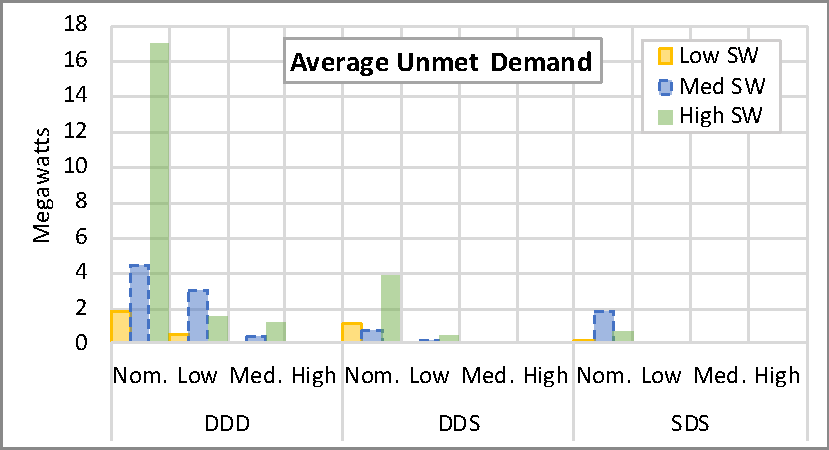
\includegraphics[trim={5mm 2mm 3mm 2mm}, clip, scale=.6]{./figures/avg_unmet_demand.pdf}
\hspace{5mm}
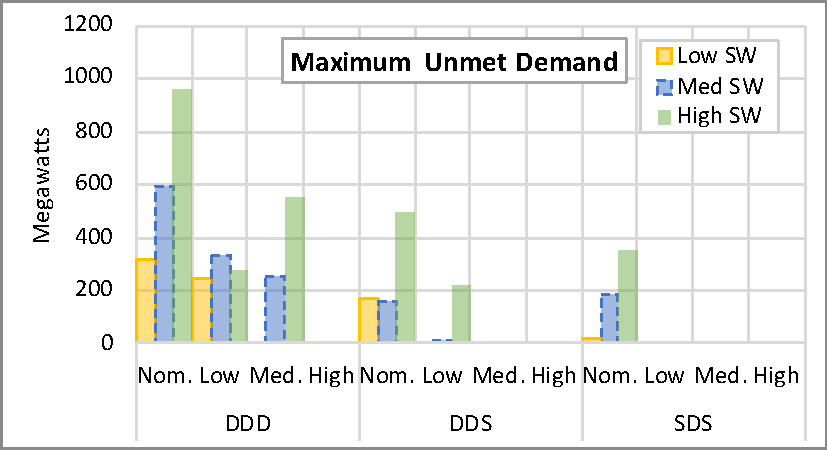
\includegraphics[trim={5mm 2mm 3mm 2mm}, clip, scale=.6]{./figures/max_unmet_demand.pdf}
\caption{Average and maximum unmet demand amounts under different reserve requirements and operations planning strategies.}
\label{sec:experiments:fig:unmet_demand}
\end{figure}

\paragraph{Reliance on ST-UC} 

\paragraph{Over Generation and Renewable Curtailment}

\subsection{Economic Impact} Figure \ref{sec:experiments:fig:avg_daily_cost} demonstrates the average daily operating-costs recorded in our experiments\footnote{This figure neglects the cost of fulfilling the unmet demands reported in the earlier sections.}. In line with our expectations, increased renewable integration leads to lower costs whereas increased reserve requirements have the opposite effect. 
\begin{figure}[h!]
\centering
% trim={<left> <lower> <right> <upper>}
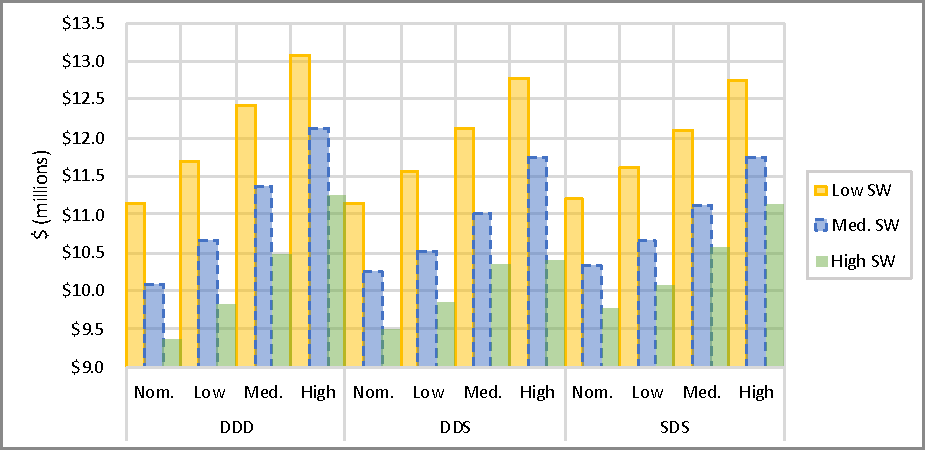
\includegraphics[trim={5mm 2mm 2mm 2mm}, clip, scale=1]{./figures/avg_daily_cost.pdf}
\caption{Average daily operating cost of the power system under different reserve requirements and operations planning strategies.}
\label{sec:experiments:fig:avg_daily_cost}
\end{figure} 

Next, we focus on cases examples where the network demand is seamlessly fulfilled. In particular, in Figure \ref{sec:experiments:fig:avg_daily_cost_demand_met}, we demonstrate the operating costs for the minimum reserve-requirement levels, subject to zero unmet demand. 
\begin{figure}[h!]
\centering
% trim={<left> <lower> <right> <upper>}
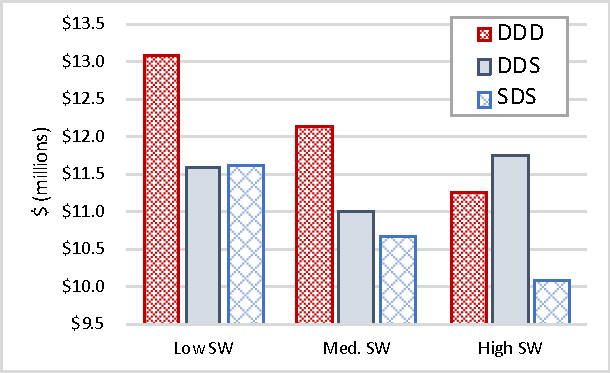
\includegraphics[trim={5mm 2mm 2mm 2mm}, clip, scale=1]{./figures/cost_vs_RI.pdf}
\caption{Average daily operating cost of the power system under all operations planning strategies (only the minimum reserve requirements leading to zero unmet demand are considered).}
\label{sec:experiments:fig:avg_daily_cost_demand_met}
\end{figure} 

\begin{figure}[h!]
\centering
% trim={<left> <lower> <right> <upper>}
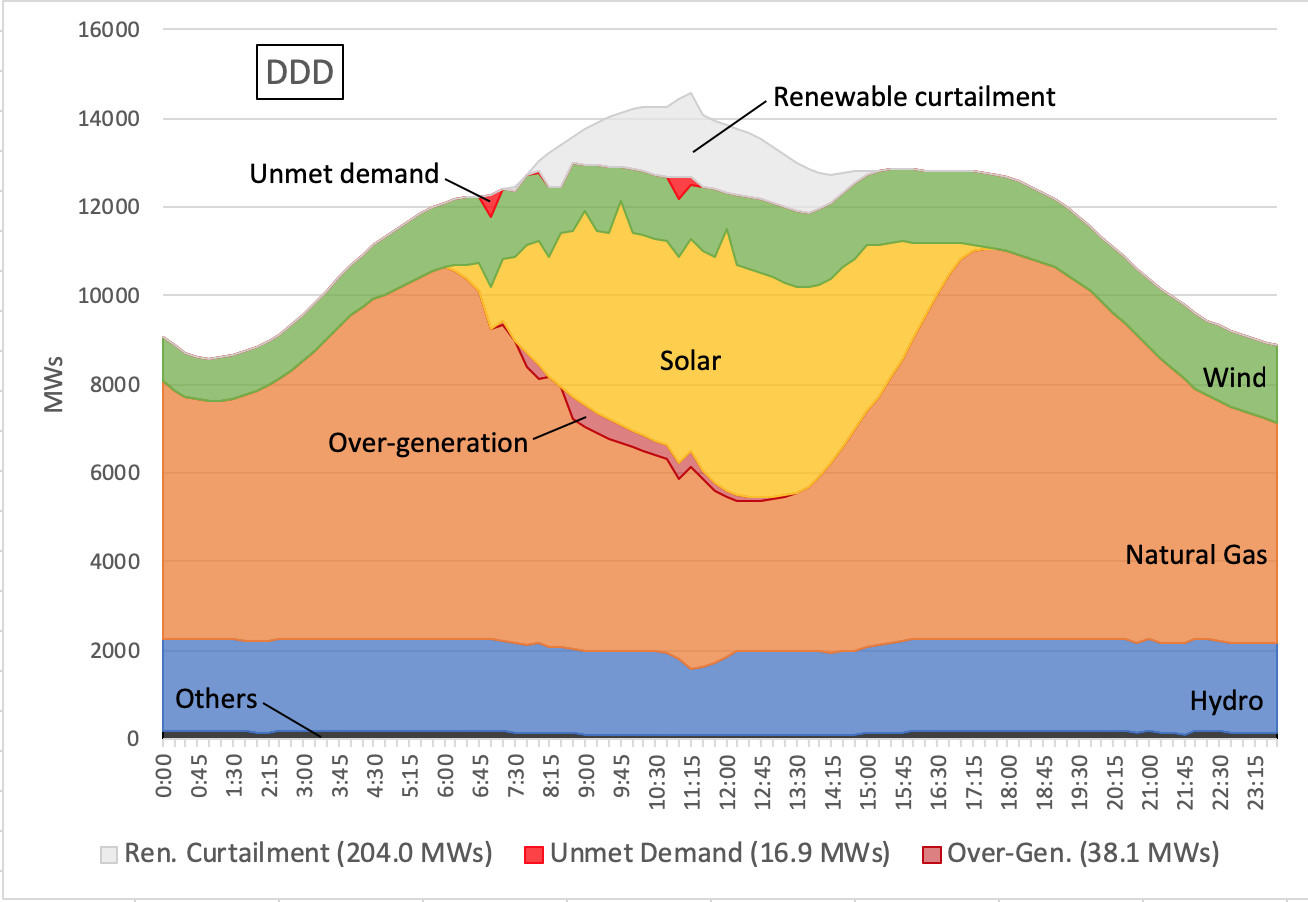
\includegraphics[trim={5mm 2mm 3mm 3mm}, clip, height=6cm]{./figures/ddd_gen_mix.png}
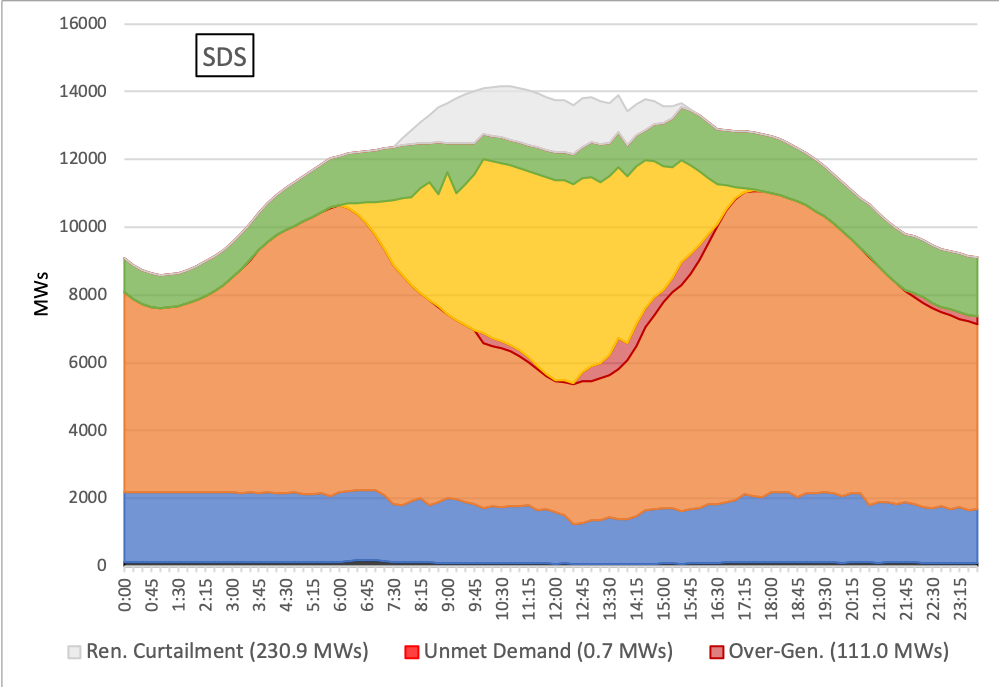
\includegraphics[trim={5mm 2mm 3mm 2mm}, clip, height=6cm]{./figures/sds_gen_mix.png}
\caption{Caption pending}
\label{sec:experiments:fig:generation_mix}
\end{figure} 


\subsection{Environmental Impact}

%It seems like stochastic models do a sufficiently good job in reducing the unmet demand in the planning process. While meeting the whole demand, stochastic models do not significantly sacrifice from costs, and may indeed perform better in certain cases. However, the cautiousness of stochastic models leads to both over-generation and renewable curtailment under high-renewable settings. This reveals a tradeoff: “greedily consuming a lot of renewable supply and not over-generating, versus risking parts of the system to shed load”.
%
%I’ve also prepared some pivot tables under high-renewable scenario. It seems like SDS (and also DDS) reduces the time-averaged commitment of natural gas generators, uses somewhat less Hydro but more Natural Gas production. This seemed a bit confusing to me: Why would you reduce the # of committed natural gas generators, but let the committed ones produce more? Because this clearly reduces your system-wide ramping capabilities? The answer, turns out, lies on the fact that most of these natural gas generators are committed in ST-UC problems. In fact, on average during a day, 15 such generators appear to be committed under DDD. The DDS and SDS reduce this statistic to 9, and 3, respectively. To put it another way, SDS clearly reduces the system's dependence on the ST-UC problems, and the reserve generators that come with it. 
%
%I feel like we have plenty of results to form a decent paper. Can we talk, sometime, what message we are trying to give the readers, and start forming a draft? Along the lines of the thesis, I’d suggest: (1) Explaining the challenges faced by the industry (unmet demand, over-generation, renewable curtailment, costs, pollutants), (2) Describe the framework for analysis, (3) Discuss our findings, (4-Appendix) Optimization methodology. In (3), we should mention that stochastic models reduce unmet demand, produce more over-generation and renewable curtailment, and give a clearer picture on achievable cost- and pollutant-prospects (because stochastic models are more reliable, less greedy).

\pagebreak
\subsubsection*{Counts of words} 
\wordcount

\bibliographystyle{apalike}
\bibliography{references}

\end{document}
